% Created by tikzDevice version 0.12.6 on 2025-04-07 13:12:00
% !TEX encoding = UTF-8 Unicode
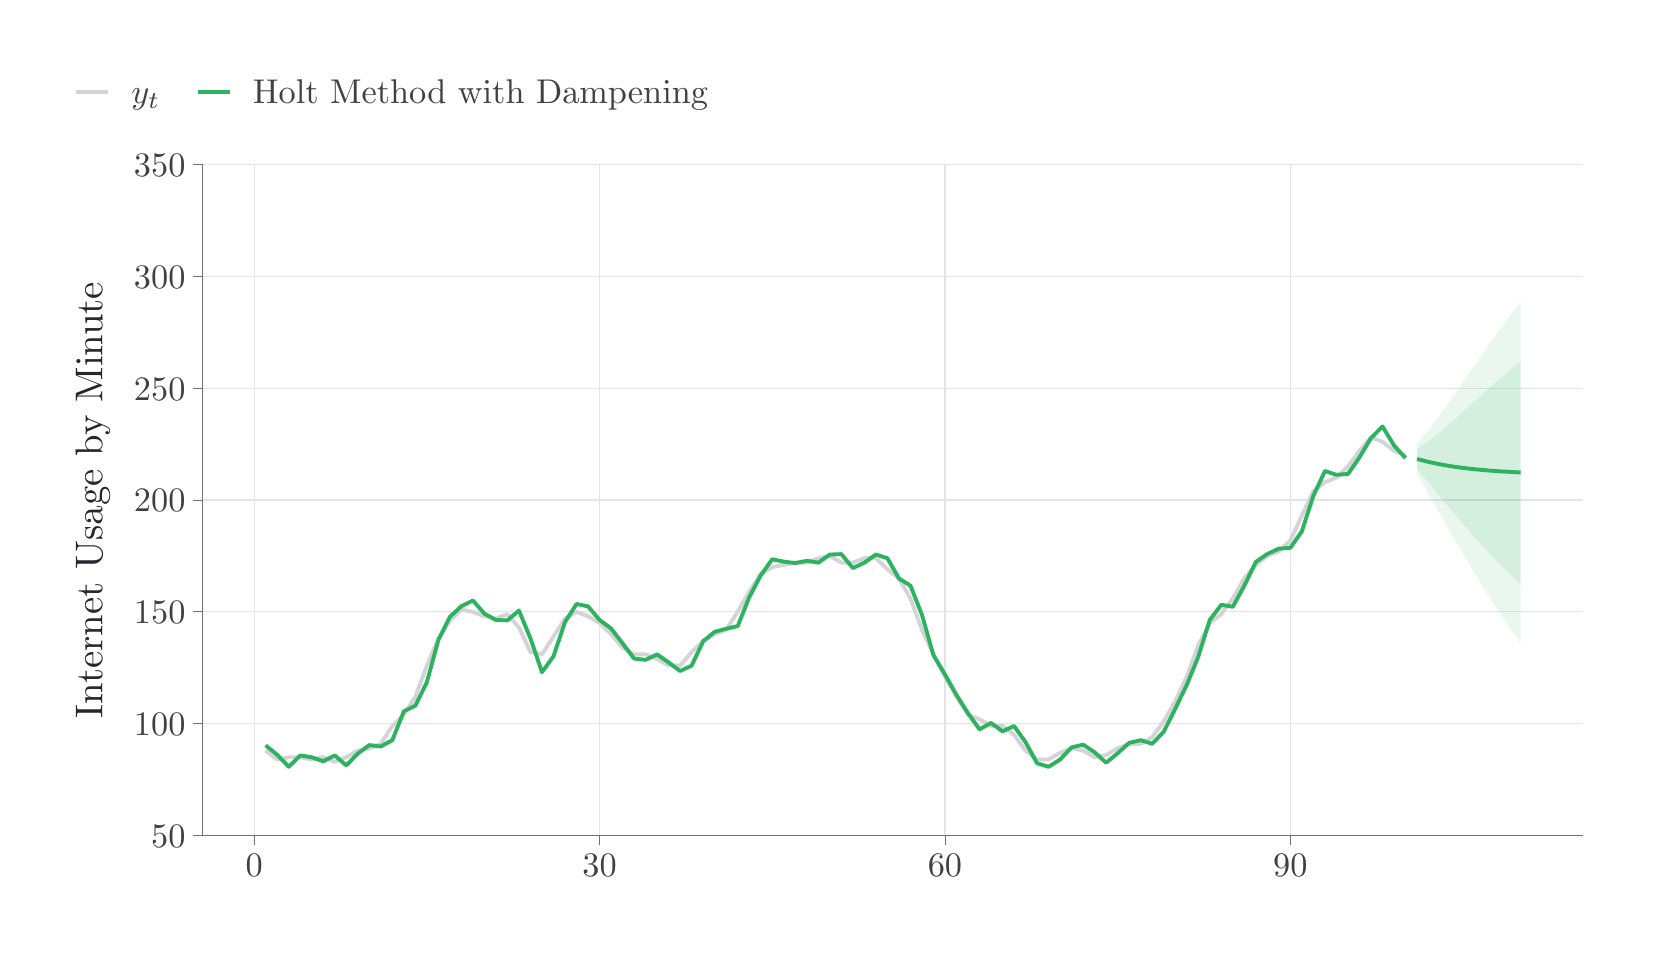
\begin{tikzpicture}[x=1pt,y=1pt]
\definecolor{fillColor}{RGB}{255,255,255}
\path[use as bounding box,fill=fillColor] (0,0) rectangle (578.16,325.21);
\begin{scope}
\path[clip] (  0.00,  0.00) rectangle (578.16,325.21);
\definecolor{drawColor}{RGB}{255,255,255}

\path[draw=drawColor,line width= 0.7pt,line join=round,line cap=round,fill=fillColor] (  0.00,  0.00) rectangle (578.16,325.21);
\end{scope}
\begin{scope}
\path[clip] ( 63.32, 33.29) rectangle (562.16,275.76);
\definecolor{drawColor}{RGB}{255,255,255}
\definecolor{fillColor}{RGB}{255,255,255}

\path[draw=drawColor,line width= 0.7pt,line join=round,line cap=round,fill=fillColor] ( 63.32, 33.29) rectangle (562.16,275.76);
\definecolor{drawColor}{RGB}{228,228,231}

\path[draw=drawColor,line width= 0.4pt,line join=round] ( 63.32, 33.29) --
	(562.16, 33.29);

\path[draw=drawColor,line width= 0.4pt,line join=round] ( 63.32, 73.70) --
	(562.16, 73.70);

\path[draw=drawColor,line width= 0.4pt,line join=round] ( 63.32,114.11) --
	(562.16,114.11);

\path[draw=drawColor,line width= 0.4pt,line join=round] ( 63.32,154.52) --
	(562.16,154.52);

\path[draw=drawColor,line width= 0.4pt,line join=round] ( 63.32,194.94) --
	(562.16,194.94);

\path[draw=drawColor,line width= 0.4pt,line join=round] ( 63.32,235.35) --
	(562.16,235.35);

\path[draw=drawColor,line width= 0.4pt,line join=round] ( 63.32,275.76) --
	(562.16,275.76);

\path[draw=drawColor,line width= 0.4pt,line join=round] ( 81.83, 33.29) --
	( 81.83,275.76);

\path[draw=drawColor,line width= 0.4pt,line join=round] (206.65, 33.29) --
	(206.65,275.76);

\path[draw=drawColor,line width= 0.4pt,line join=round] (331.46, 33.29) --
	(331.46,275.76);

\path[draw=drawColor,line width= 0.4pt,line join=round] (456.28, 33.29) --
	(456.28,275.76);
\definecolor{drawColor}{RGB}{212,212,216}

\path[draw=drawColor,line width= 1.4pt,line join=round] ( 85.99, 64.00) --
	( 90.15, 60.77) --
	( 94.31, 61.57) --
	( 98.48, 61.57) --
	(102.64, 60.77) --
	(106.80, 61.57) --
	(110.96, 59.96) --
	(115.12, 61.57) --
	(119.28, 64.00) --
	(123.44, 64.81) --
	(127.60, 66.42) --
	(131.76, 72.89) --
	(135.92, 76.93) --
	(140.08, 83.40) --
	(144.24, 94.71) --
	(148.40,104.41) --
	(152.56,110.88) --
	(156.72,114.92) --
	(160.88,114.11) --
	(165.04,112.49) --
	(169.20,111.69) --
	(173.36,113.30) --
	(177.52,108.45) --
	(181.68, 99.56) --
	(185.85, 98.75) --
	(190.01,105.22) --
	(194.17,111.69) --
	(198.33,114.11) --
	(202.49,112.49) --
	(206.65,110.07) --
	(210.81,106.03) --
	(214.97,101.18) --
	(219.13, 98.75) --
	(223.29, 98.75) --
	(227.45, 97.14) --
	(231.61, 94.71) --
	(235.77, 94.71) --
	(239.93, 99.56) --
	(244.09,103.60) --
	(248.25,106.03) --
	(252.41,107.64) --
	(256.57,114.11) --
	(260.73,121.39) --
	(264.89,127.85) --
	(269.05,130.28) --
	(273.22,131.08) --
	(277.38,131.89) --
	(281.54,131.89) --
	(285.70,133.51) --
	(289.86,134.32) --
	(294.02,131.89) --
	(298.18,131.89) --
	(302.34,133.51) --
	(306.50,133.51) --
	(310.66,129.47) --
	(314.82,126.23) --
	(318.98,118.96) --
	(323.14,107.64) --
	(327.30, 98.75) --
	(331.46, 90.67) --
	(335.62, 83.40) --
	(339.78, 76.93) --
	(343.94, 75.31) --
	(348.10, 72.89) --
	(352.26, 72.89) --
	(356.42, 69.66) --
	(360.58, 64.00) --
	(364.75, 60.77) --
	(368.91, 60.77) --
	(373.07, 63.19) --
	(377.23, 64.81) --
	(381.39, 64.00) --
	(385.55, 61.57) --
	(389.71, 62.38) --
	(393.87, 64.81) --
	(398.03, 66.42) --
	(402.19, 66.42) --
	(406.35, 68.85) --
	(410.51, 74.51) --
	(414.67, 81.78) --
	(418.83, 90.67) --
	(422.99,101.99) --
	(427.15,110.07) --
	(431.31,113.30) --
	(435.47,118.96) --
	(439.63,126.23) --
	(443.79,131.08) --
	(447.95,134.32) --
	(452.12,135.93) --
	(456.28,139.97) --
	(460.44,148.87) --
	(464.60,157.76) --
	(468.76,160.99) --
	(472.92,162.61) --
	(477.08,166.65) --
	(481.24,172.31) --
	(485.40,177.15) --
	(489.56,175.54) --
	(493.72,172.31) --
	(497.88,170.69);
\definecolor{drawColor}{RGB}{45,178,95}

\path[draw=drawColor,line width= 1.4pt,line join=round] ( 85.99, 65.89) --
	( 90.15, 62.46) --
	( 94.31, 58.14) --
	( 98.48, 62.22) --
	(102.64, 61.58) --
	(106.80, 60.11) --
	(110.96, 62.23) --
	(115.12, 58.65) --
	(119.28, 62.88) --
	(123.44, 65.97) --
	(127.60, 65.47) --
	(131.76, 67.74) --
	(135.92, 78.14) --
	(140.08, 80.23) --
	(144.24, 88.66) --
	(148.40,103.92) --
	(152.56,112.31) --
	(156.72,116.15) --
	(160.88,118.22) --
	(165.04,113.46) --
	(169.20,111.18) --
	(173.36,111.03) --
	(177.52,114.61) --
	(181.68,104.52) --
	(185.85, 92.33) --
	(190.01, 98.08) --
	(194.17,110.47) --
	(198.33,116.95) --
	(202.49,116.10) --
	(206.65,111.19) --
	(210.81,108.10) --
	(214.97,102.74) --
	(219.13, 97.23) --
	(223.29, 96.77) --
	(227.45, 98.75) --
	(231.61, 95.83) --
	(235.77, 92.74) --
	(239.93, 94.71) --
	(244.09,103.50) --
	(248.25,106.90) --
	(252.41,108.01) --
	(256.57,108.96) --
	(260.73,119.37) --
	(264.89,127.31) --
	(269.05,133.12) --
	(273.22,132.26) --
	(277.38,131.75) --
	(281.54,132.55) --
	(285.70,131.89) --
	(289.86,134.82) --
	(294.02,134.98) --
	(298.18,129.93) --
	(302.34,131.89) --
	(306.50,134.82) --
	(310.66,133.51) --
	(314.82,126.19) --
	(318.98,123.60) --
	(323.14,113.05) --
	(327.30, 98.44) --
	(331.46, 91.51) --
	(335.62, 84.09) --
	(339.78, 77.47) --
	(343.94, 71.66) --
	(348.10, 73.99) --
	(352.26, 70.92) --
	(356.42, 72.88) --
	(360.58, 67.03) --
	(364.75, 59.40) --
	(368.91, 58.13) --
	(373.07, 60.76) --
	(377.23, 65.16) --
	(381.39, 66.13) --
	(385.55, 63.35) --
	(389.71, 59.60) --
	(393.87, 63.03) --
	(398.03, 66.78) --
	(402.19, 67.74) --
	(406.35, 66.43) --
	(410.51, 70.82) --
	(414.67, 79.11) --
	(418.83, 87.70) --
	(422.99, 97.91) --
	(427.15,111.20) --
	(431.31,116.66) --
	(435.47,115.95) --
	(439.63,123.56) --
	(443.79,132.16) --
	(447.95,135.04) --
	(452.12,136.95) --
	(456.28,137.25) --
	(460.44,143.26) --
	(464.60,156.10) --
	(468.76,165.00) --
	(472.92,163.64) --
	(477.08,163.93) --
	(481.24,169.93) --
	(485.40,176.91) --
	(489.56,181.11) --
	(493.72,174.24) --
	(497.88,169.68);

\path[draw=drawColor,line width= 1.4pt,line join=round] (502.04,169.37) --
	(506.20,168.29) --
	(510.36,167.42) --
	(514.52,166.70) --
	(518.68,166.12) --
	(522.84,165.64) --
	(527.00,165.26) --
	(531.16,164.94) --
	(535.32,164.69) --
	(539.49,164.48);
\definecolor{fillColor}{RGB}{45,178,95}

\path[fill=fillColor,fill opacity=0.10] (502.04,172.99) --
	(506.20,175.79) --
	(510.36,179.10) --
	(514.52,182.69) --
	(518.68,186.41) --
	(522.84,190.19) --
	(527.00,193.95) --
	(531.16,197.66) --
	(535.32,201.29) --
	(539.49,204.83) --
	(539.49,124.12) --
	(535.32,128.08) --
	(531.16,132.23) --
	(527.00,136.57) --
	(522.84,141.10) --
	(518.68,145.82) --
	(514.52,150.72) --
	(510.36,155.73) --
	(506.20,160.80) --
	(502.04,165.75) --
	cycle;

\path[] (502.04,172.99) --
	(506.20,175.79) --
	(510.36,179.10) --
	(514.52,182.69) --
	(518.68,186.41) --
	(522.84,190.19) --
	(527.00,193.95) --
	(531.16,197.66) --
	(535.32,201.29) --
	(539.49,204.83);

\path[] (539.49,124.12) --
	(535.32,128.08) --
	(531.16,132.23) --
	(527.00,136.57) --
	(522.84,141.10) --
	(518.68,145.82) --
	(514.52,150.72) --
	(510.36,155.73) --
	(506.20,160.80) --
	(502.04,165.75);

\path[fill=fillColor,fill opacity=0.10] (502.04,174.91) --
	(506.20,179.76) --
	(510.36,185.28) --
	(514.52,191.15) --
	(518.68,197.16) --
	(522.84,203.18) --
	(527.00,209.14) --
	(531.16,214.98) --
	(535.32,220.67) --
	(539.49,226.20) --
	(539.49,102.75) --
	(535.32,108.70) --
	(531.16,114.91) --
	(527.00,121.38) --
	(522.84,128.11) --
	(518.68,135.08) --
	(514.52,142.25) --
	(510.36,149.55) --
	(506.20,156.83) --
	(502.04,163.83) --
	cycle;

\path[] (502.04,174.91) --
	(506.20,179.76) --
	(510.36,185.28) --
	(514.52,191.15) --
	(518.68,197.16) --
	(522.84,203.18) --
	(527.00,209.14) --
	(531.16,214.98) --
	(535.32,220.67) --
	(539.49,226.20);

\path[] (539.49,102.75) --
	(535.32,108.70) --
	(531.16,114.91) --
	(527.00,121.38) --
	(522.84,128.11) --
	(518.68,135.08) --
	(514.52,142.25) --
	(510.36,149.55) --
	(506.20,156.83) --
	(502.04,163.83);
\end{scope}
\begin{scope}
\path[clip] (  0.00,  0.00) rectangle (578.16,325.21);
\definecolor{drawColor}{RGB}{113,113,122}

\path[draw=drawColor,line width= 0.3pt,line join=round] ( 63.32, 33.29) --
	( 63.32,275.76);
\end{scope}
\begin{scope}
\path[clip] (  0.00,  0.00) rectangle (578.16,325.21);
\definecolor{drawColor}{RGB}{63,63,70}

\node[text=drawColor,anchor=base east,inner sep=0pt, outer sep=0pt, scale=  1.24] at ( 57.02, 29.00) {50};

\node[text=drawColor,anchor=base east,inner sep=0pt, outer sep=0pt, scale=  1.24] at ( 57.02, 69.41) {100};

\node[text=drawColor,anchor=base east,inner sep=0pt, outer sep=0pt, scale=  1.24] at ( 57.02,109.83) {150};

\node[text=drawColor,anchor=base east,inner sep=0pt, outer sep=0pt, scale=  1.24] at ( 57.02,150.24) {200};

\node[text=drawColor,anchor=base east,inner sep=0pt, outer sep=0pt, scale=  1.24] at ( 57.02,190.65) {250};

\node[text=drawColor,anchor=base east,inner sep=0pt, outer sep=0pt, scale=  1.24] at ( 57.02,231.06) {300};

\node[text=drawColor,anchor=base east,inner sep=0pt, outer sep=0pt, scale=  1.24] at ( 57.02,271.48) {350};
\end{scope}
\begin{scope}
\path[clip] (  0.00,  0.00) rectangle (578.16,325.21);
\definecolor{drawColor}{RGB}{113,113,122}

\path[draw=drawColor,line width= 0.3pt,line join=round] ( 59.82, 33.29) --
	( 63.32, 33.29);

\path[draw=drawColor,line width= 0.3pt,line join=round] ( 59.82, 73.70) --
	( 63.32, 73.70);

\path[draw=drawColor,line width= 0.3pt,line join=round] ( 59.82,114.11) --
	( 63.32,114.11);

\path[draw=drawColor,line width= 0.3pt,line join=round] ( 59.82,154.52) --
	( 63.32,154.52);

\path[draw=drawColor,line width= 0.3pt,line join=round] ( 59.82,194.94) --
	( 63.32,194.94);

\path[draw=drawColor,line width= 0.3pt,line join=round] ( 59.82,235.35) --
	( 63.32,235.35);

\path[draw=drawColor,line width= 0.3pt,line join=round] ( 59.82,275.76) --
	( 63.32,275.76);
\end{scope}
\begin{scope}
\path[clip] (  0.00,  0.00) rectangle (578.16,325.21);
\definecolor{drawColor}{RGB}{113,113,122}

\path[draw=drawColor,line width= 0.3pt,line join=round] ( 63.32, 33.29) --
	(562.16, 33.29);
\end{scope}
\begin{scope}
\path[clip] (  0.00,  0.00) rectangle (578.16,325.21);
\definecolor{drawColor}{RGB}{113,113,122}

\path[draw=drawColor,line width= 0.3pt,line join=round] ( 81.83, 29.79) --
	( 81.83, 33.29);

\path[draw=drawColor,line width= 0.3pt,line join=round] (206.65, 29.79) --
	(206.65, 33.29);

\path[draw=drawColor,line width= 0.3pt,line join=round] (331.46, 29.79) --
	(331.46, 33.29);

\path[draw=drawColor,line width= 0.3pt,line join=round] (456.28, 29.79) --
	(456.28, 33.29);
\end{scope}
\begin{scope}
\path[clip] (  0.00,  0.00) rectangle (578.16,325.21);
\definecolor{drawColor}{RGB}{63,63,70}

\node[text=drawColor,anchor=base,inner sep=0pt, outer sep=0pt, scale=  1.24] at ( 81.83, 18.42) {0};

\node[text=drawColor,anchor=base,inner sep=0pt, outer sep=0pt, scale=  1.24] at (206.65, 18.42) {30};

\node[text=drawColor,anchor=base,inner sep=0pt, outer sep=0pt, scale=  1.24] at (331.46, 18.42) {60};

\node[text=drawColor,anchor=base,inner sep=0pt, outer sep=0pt, scale=  1.24] at (456.28, 18.42) {90};
\end{scope}
\begin{scope}
\path[clip] (  0.00,  0.00) rectangle (578.16,325.21);
\definecolor{drawColor}{RGB}{39,39,42}

\node[text=drawColor,rotate= 90.00,anchor=base,inner sep=0pt, outer sep=0pt, scale=  1.40] at ( 27.00,154.52) {Internet Usage by Minute};
\end{scope}
\begin{scope}
\path[clip] (  0.00,  0.00) rectangle (578.16,325.21);
\definecolor{drawColor}{RGB}{255,255,255}
\definecolor{fillColor}{RGB}{255,255,255}

\path[draw=drawColor,line width= 0.7pt,line join=round,line cap=round,fill=fillColor] ( 16.00,289.76) rectangle (246.35,309.22);
\end{scope}
\begin{scope}
\path[clip] (  0.00,  0.00) rectangle (578.16,325.21);
\definecolor{drawColor}{RGB}{255,255,255}
\definecolor{fillColor}{RGB}{255,255,255}

\path[draw=drawColor,line width= 0.7pt,line join=round,line cap=round,fill=fillColor] ( 16.00,294.76) rectangle ( 30.45,309.22);
\end{scope}
\begin{scope}
\path[clip] (  0.00,  0.00) rectangle (578.16,325.21);
\definecolor{drawColor}{RGB}{212,212,216}

\path[draw=drawColor,line width= 1.4pt,line join=round] ( 17.45,301.99) -- ( 29.01,301.99);
\end{scope}
\begin{scope}
\path[clip] (  0.00,  0.00) rectangle (578.16,325.21);
\definecolor{drawColor}{RGB}{255,255,255}
\definecolor{fillColor}{RGB}{255,255,255}

\path[draw=drawColor,line width= 0.7pt,line join=round,line cap=round,fill=fillColor] ( 59.93,294.76) rectangle ( 74.39,309.22);
\end{scope}
\begin{scope}
\path[clip] (  0.00,  0.00) rectangle (578.16,325.21);
\definecolor{drawColor}{RGB}{45,178,95}

\path[draw=drawColor,line width= 1.4pt,line join=round] ( 61.38,301.99) -- ( 72.94,301.99);
\end{scope}
\begin{scope}
\path[clip] (  0.00,  0.00) rectangle (578.16,325.21);
\definecolor{drawColor}{RGB}{63,63,70}

\node[text=drawColor,anchor=base west,inner sep=0pt, outer sep=0pt, scale=  1.24] at ( 37.45,297.70) {$y_t$};
\end{scope}
\begin{scope}
\path[clip] (  0.00,  0.00) rectangle (578.16,325.21);
\definecolor{drawColor}{RGB}{63,63,70}

\node[text=drawColor,anchor=base west,inner sep=0pt, outer sep=0pt, scale=  1.24] at ( 81.39,297.70) {Holt Method with Dampening};
\end{scope}
\end{tikzpicture}
